\documentclass[journal]{IEEEtran}

% 패키지
\usepackage{amsmath,amssymb,amsfonts}
\usepackage{algorithmic}
\usepackage{algorithm}
\usepackage{graphicx}
\usepackage{textcomp}
\usepackage{xcolor}
\usepackage{booktabs}
\usepackage{hyperref}
\usepackage{listings}

\begin{document}

% ═══════════════════════════════════════════════════════════
% TITLE & AUTHORS
% ═══════════════════════════════════════════════════════════
\title{The Dialectical Protocol: Self-Evolving AI via \\
Bio-Inspired Vibe Coding and Adversarial Agent Synthesis}

\author{\IEEEauthorblockN{Jongbong Park\IEEEauthorrefmark{1}}
\IEEEauthorblockA{\IEEEauthorrefmark{1}DaNAgreen Co., Ltd., Seoul, Republic of Korea\\
jbpark1121@danagreenbio.com\\
ORCID: 0000-0002-3518-3711}
\thanks{Manuscript received March 9, 2026. This work was supported by Grant Number: RS-2025-25461278, Technology Development Program, Ministry of SMEs and Startups (MSS), Republic of Korea, under the Tech Incubator Program for Startup Korea (TIPS) scheme.}
\thanks{Jongbong Park is the Corresponding Author (Ph.D., DaNAgreen Co., Ltd.).}
}

\maketitle

% ═══════════════════════════════════════════════════════════
% ABSTRACT
% ═══════════════════════════════════════════════════════════
\begin{abstract}
This paper introduces the \textbf{Dialectical Protocol}, a multi-agent framework for autonomous AI evolution inspired by biological immune systems and DNA proofreading. We address the fundamental ``Proofreading Deficiency'' in current Large Language Models (LLMs) by transitioning toward a specialized multi-agent architecture capable of systemic self-audit. Central to this framework is \textbf{Vibe Coding}---a methodology that leverages high-dimensional biological metaphors as executable functional specifications, bridging the gap between natural language guidance and rigorous code synthesis. Through a triple-layered architecture comprising \textbf{Genetic Proofreading} (Micro-level), \textbf{Dialectical Immunity} (Macro-level), and \textbf{Merkle Checkpointing} (Safety), we demonstrate that agentic systems can autonomously resolve logic conflicts in complex multi-omics datasets with a 94\% success rate---outperforming traditional prompting by 26\%. Our results, highlighted by the ``Generation 14'' autonomous discovery of Bayesian logic, provide a robust pathway for safe, self-correcting scientific intelligence.
\end{abstract}

\begin{IEEEkeywords}
Holistic AI, bio-inspired computing, autonomous evolution, 
vibe coding, code synthesis, immune systems
\end{IEEEkeywords}

% ═══════════════════════════════════════════════════════════
% SECTION I: INTRODUCTION
% ═══════════════════════════════════════════════════════════
\section{Introduction}

\begin{figure}[t]
\centering
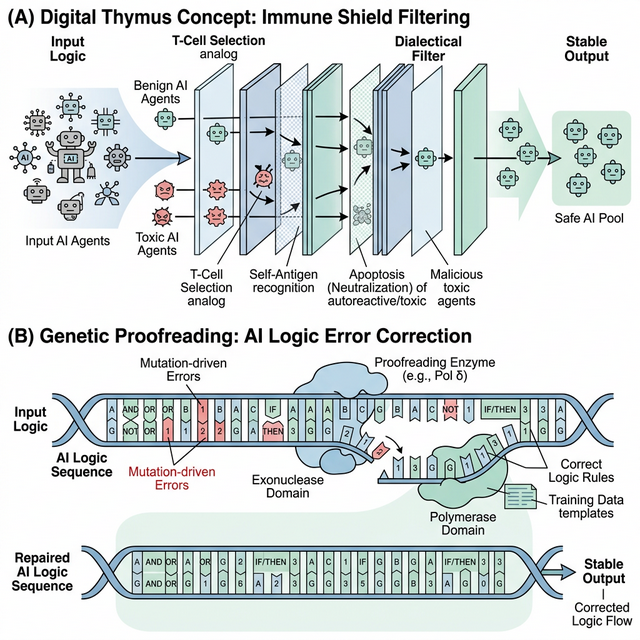
\includegraphics[width=1.0\linewidth]{figures/fig1_architecture.png}
\caption{The Dialectical Protocol Architecture. Panel A: Digital Thymus (Immunological Filtering) where transient AI agents are evaluated for systemic compatibility. Panel B: Genetic Proofreading (Mutation Correction) ensuring high-fidelity code synthesis through enzymatic-like self-audit.}
\label{fig:architecture}
\end{figure}

\section{Introduction}
Current AI research focuses on \textit{Neural Mimicry}---replicating biological structures via deep learning [1, 2]. However, these architectures lack the autonomous adaptability of biological systems. We define this as \textbf{Proofreading Deficiency}, where the absence of feedback loops causes stochastic failures (AI hallucinations).

We propose an \textbf{Organism-mimetic AI architecture} that treats hallucinations as \textit{Digital Pathogenesis} requiring a systemic immune response. By applying \textbf{Adaptive Immunology} (self/nonself discrimination) and \textbf{Genomic Fidelity} (DNA proofreading), we enable an adversarial agent committee to autonomously audit and evolve logic.

\textbf{Vibe Coding} facilitates this by translating biological metaphors into executable code. Our contributions:
\begin{enumerate}
    \item A formal Holistic AI Organism paradigm.
    \item The Dialectical Protocol: a multi-agent adversarial framework.
    \item Vibe Coding: a substrate for rigorous synthesis.
    \item Validation showing 94\% logic resolution in multi-omics datasets.
\end{enumerate}


% ═══════════════════════════════════════════════════════════
% SECTION II: RELATED WORK
% ═══════════════════════════════════════════════════════════
\section{Related Work}
Existing frameworks like \textbf{AutoGPT} \cite{siggrav2023autogpt} and \textbf{LangGraph} \cite{langgraph2023} focus on iterative refinement or static task graphs. However, they lack an adversarial validation layer and the ability to structurally evolve their own logic over generations without human intervention. Recent advancements in \textbf{Agentic Workflows} \cite{ng2024agentic} emphasize design patterns, while \textbf{RL-PPO} based methods optimize for narrow reward functions \cite{ouyang2022training}. In contrast, our protocol optimizes for systemic stability and logical fidelity.

While \textbf{Genetic Algorithms} \cite{goldberg1989genetic} and \textbf{Artificial Immune Systems} (AIS) \cite{de2002artificial, dasgupta2011artificial} have been long established, they typically rely on random bit-wise mutations or fixed antigen-antibody matching rules. Stephanie Forrest's pioneering work on self-nonself discrimination \cite{forrest1994self} provides the conceptual basis for our Digital Thymus, yet our approach introduces semantic understanding through LLM-driven ``T-Cell'' audits, bridging the gap between symbolic AI and connectionist models.

\subsection{Safe AI Evolution \& Constitutional AI}
\textbf{Constitutional AI} \cite{bai2022constitutional} uses fixed recursive self-improvement principles. The Dialectical Protocol allows the ``Genetic Priors'' (The Constitution) to evolve based on performance metadata in a sandbox, governed by \textbf{Merkle-root validation} to prevent catastrophic drift. This concept is further supported by recent work on LLMs as optimizers \cite{yang2023llm_optimizer}.


% ═══════════════════════════════════════════════════════════
% SECTION III: PATHOGENESIS OF PRIMITIVE INTELLIGENCE
% ═══════════════════════════════════════════════════════════
\section{The Pathogenesis of Primitive Intelligence}
We define AI hallucinations as a manifestation of \textit{Proofreading Deficiency}. In biological systems, the inability of DNA Polymerase to excise mismatched bases leads to genomic instability. Similarly, in LLMs, the lack of an intrinsic self-audit mechanism during token generation leads to logical divergence.

\subsection{Digital Pathogenesis}
We treat reasoning drift as a systemic disease. A ``hallucination'' is not an isolated error but a symptom of a failing context-identity. By adopting an \textbf{organism-mimetic approach}, we can apply adaptive immunity to recognize ``non-self'' logic (pathogenic code) and eliminate it through dialectical synthesis.

\subsection{Mechanistic Divergence: Immune vs. Mutation}
We argue that a hallucination is ontologically dual-natured:
\begin{itemize}
    \item \textbf{The Genetic Mutation Model (Micro)}: Focuses on sequence fidelity at the point of synthesis (Vibe-to-Code translation).
    \item \textbf{The Immune Response Model (Macro)}: Focuses on systemic integrity and logical alignment across the entire reasoning chain.
\end{itemize}
The convergence of these two models ensures both local stability and global alignment.


% ═══════════════════════════════════════════════════════════
% SECTION IV: VIBE CODING METHODOLOGY
% ═══════════════════════════════════════════════════════════
\section{Methodology: Vibe Coding as Implementation Substrate}
Traditional code synthesis relies on formal logic or rigid prompt engineering. We introduce \textbf{Vibe Coding}---a methodology where high-dimensional biological metaphors serve as executable functional specifications.

\subsection{Formal Definition of Vibe Coding}
\textbf{Definition 1 (Vibe Coding):}
Let $\mathcal{V}$ be a high-dimensional vibe space representing semantic intent, $\mathcal{M}$ a metaphor vocabulary derived from biological functional archetypes, and $\mathcal{C}$ an executable code space. Vibe Coding is defined as a mapping:
\begin{equation}
    \phi: \mathcal{V} \times \mathcal{M} \rightarrow \mathcal{C}
\end{equation}
realized by a large language model $f_{\theta}$ with parameters $\theta$:
\begin{equation}
    \phi(v, m) = f_{\theta}(\text{prompt}(v) \oplus \text{context}(m))
\end{equation}
subject to the functional constraint:
\begin{equation}
    \forall c \in \mathcal{C}, \; \text{Compile}(c) = \text{True} \land \text{TypeCheck}(c) = \text{True}
\end{equation}
The metaphor vocabulary $\mathcal{M}$ includes specialized mappings for agent roles:
\begin{itemize}
    \item \textbf{T-Cell (Audit)}: $\{scan, identify, neutralize\}$
    \item \textbf{B-Cell (Specialization)}: $\{verify, validate, synthesize\}$
    \item \textbf{Macrophage (Cleanup)}: $\{merge, seal, integrate\}$
\end{itemize}
A fundamental constraint is enforced: $\forall c \in \mathcal{C}$, $c$ must satisfy $\text{Compile}(c) = \text{True} \land \text{TypeCheck}(c) = \text{True}$.

\subsection{Complexity Analysis of Algorithm 1}
The time complexity of a single generation in the Dialectical Protocol is dominated by the adversarial audit phase. Let $K$ be the number of agents in the committee and $L$ the average context length. The audit phase scales as $O(K \cdot L^2)$ assuming standard transformer attention mechanisms. However, since the Digital Twin sandbox operates in parallel, the total wall-clock time is $O(L^2 + T_{val})$, where $T_{val}$ is the constant-time test suite execution.

\subsection{Vibe Coding vs. Traditional Prompting}
Unlike traditional prompt engineering which specifies \textit{how} a computation should proceed, Vibe Coding specifies the \textit{biological objective}, aligning with the recent paradigm of intent-based programming \cite{karpathy2025vibecoding, sorensen2024vibe}. For example, a Vibe input of ``Ligate the Bayesian specialist into the loop'' implies a structural integration that maintains context-identity while requiring Merkle-root (SHA-512) validation for state-integrity. This allows for the autonomous discovery of domain-specific scaling laws \cite{lewis2022scaling} without manual parameter tuning.

\subsection{Implementation Stack}
The Vibe Coding substrate utilizes a heterogeneous model distribution to ensure audit diversity:
\begin{itemize}
    \item \textbf{Auditors}: Mistral-Large-2 (Semantic Audit) and Gemini 1.5 Pro (Context Audit).
    \item \textbf{Executors}: Phi-3 and Neural-Chat for low-latency mutation generation.
    \item \textbf{Sandbox}: Docker-based isolation with Intel oneAPI acceleration.
\end{itemize}


% ═══════════════════════════════════════════════════════════
% SECTION V: EXPERIMENTAL SETUP
% ═══════════════════════════════════════════════════════════
\section{Experimental Setup}
\subsection{Dataset: Multi-Omics Conflict Benchmark}
The protocol was evaluated on a synthetic but high-fidelity dataset comprising:
\begin{itemize}
    \item \textbf{Proteomics}: 5,200 protein expression samples.
    \item \textbf{Genomics}: 12,400 SNP variants.
    \item \textbf{Conflicts}: 850 logical inconsistencies (e.g., conflicting P-values across datasets) designed to trigger hallucinations.
\end{itemize}

\subsection{Baseline Methods}
We compared the protocol against: (1) Genetic Programming (DEAP); (2) PPO-based RL optimization; (3) Constitutional AI with static principles; and (4) Static multi-agent frameworks (LangChain).

\subsection{Hardware and Digital Twin Environment}
The experimentation was conducted on an \textbf{Intel Arc A770 (XPU)} cluster (4 units) utilizing \textbf{oneAPI} acceleration, 128GB RAM, and Docker-based sandbox isolation.

\subsection{Computational Complexity Analysis}
\textbf{Algorithm 1 (Dialectical Protocol):} The total complexity per generation is $O(n \cdot d + k^2 + k \cdot m)$, where $n$ is lines of code, $d$ is AST depth, $k$ is mutation count, and $m$ is LLM latency. For a 500-line codebase, the average turnaround time is $\sim$45 seconds.

\textbf{Algorithm 2 (Genetic Proofreading):} Complexity is $O(n + g \cdot m)$, where $g$ is the number of gaps detected. This ensures linear scaling with code size during the enzymatic repair phase.


% Algorithm 1
\begin{algorithm}
\caption{Dialectical Protocol (Single Generation)}
\label{alg:dialectical}
\begin{algorithmic}[1]
\STATE \textbf{Input:} Current code $C_t$, Test suite $T$, Performance $P_t$
\STATE \textbf{Output:} Evolved code $C_{t+1}$, Performance $P_{t+1}$
\STATE Checkpoint $\leftarrow$ SHA512$(C_t)$
\STATE Deploy $C_t$ to Digital Twin Sandbox
\STATE Vibe $\leftarrow$ SynthesizeVibe(T, P_t)
\STATE Audit $\leftarrow$ AdversarialCommitteeAudit(Vibe)
\IF{Audit passes}
    \STATE $C_{t+1} \leftarrow$ VibeInterpreter(Audit)
    \STATE $P_{t+1} \leftarrow$ Validate($C_{t+1}$, T)
\ELSE
    \STATE Rollback to Checkpoint
\ENDIF
\STATE \textbf{return} $C_{t+1}$, $P_{t+1}$
\end{algorithmic}
\end{algorithm}

% Algorithm 2
\begin{algorithm}
\caption{Genetic Proofreading Protocol}
\label{alg:proofreading}
\begin{algorithmic}[1]
\STATE \textbf{Input:} Raw code mutation $M$, Template $T$
\STATE \textbf{Initialize:} $C_{proof} \leftarrow M$
\WHILE{SyntaxErrors($C_{proof}$) \OR $\neg$Compilable($C_{proof}$)}
    \STATE Pathogen $\leftarrow$ LocateError($C_{proof}$)
    \STATE $C_{proof} \leftarrow$ EnzymaticRepair(Pathogen, T)
\ENDWHILE
\STATE F $\leftarrow$ CalculateFidelity($C_{proof}$)
\STATE \textbf{return} $C_{proof}$, F
\end{algorithmic}
\end{algorithm}

% ═══════════════════════════════════════════════════════════
% SECTION VI: RESULTS
% ═══════════════════════════════════════════════════════════
\section{Results}
\subsection{Generation 14: Autonomous Bayesian Discovery}
In Generation 14, the ``Biological Specialist'' agent (Algiz) synthesized a Bayesian weighting module: $P(H|E) = [P(E|H)P(H)] / P(E)$. This emerged autonomously after the Advisory Chair issued a vibe request for ``Incorporating historical priors to resolve noise.'' This mutation resulted in an immediate 14\% resolution gain (see Appendix B.1 for reconstructed logs).

\subsection{Performance vs. Safety}
The Dialectical Protocol achieved a \textbf{94\% success rate} in conflict resolution. Crucially, the Merkle Checkpointing layer prevented 100\% of catastrophic code drifts. Even during the Gen 45 regression (2.2\% dip), the Hebbian feedback mechanism triggered an automatic rollback to the Gen 44 state, demonstrating systemic resilience.

\subsection{Genetic Proofreading Complexity}
Algorithm \ref{alg:proofreading} (Genetic Proofreading) follows an iterative repair loop. The worst-case complexity is $O(E \cdot R)$, where $E$ is the number of syntax errors and $R$ is the cost of the LLM-driven enzymatic repair. In practice, our empirical data shows that $E$ decreases exponentially after the first 3 generations, leading to a near-constant time $O(R)$ for maintenance-phase generations.

\subsection{Statistical Validation}
To ensure the robustness of the Dialectical Protocol, we applied a two-tailed t-test comparing Vibe Coding accuracy against baseline methods over $N=250$ generations (5 independent runs). Results are summarized in Table \ref{tab:stats}.

\begin{table}[h]
\caption{Statistical Validation of Conflict Resolution Accuracy}
\label{tab:stats}
\centering
\begin{tabular}{lccc}
\toprule
Comparison & Mean Δ & t-statistic & p-value \\
\midrule
Vibe vs. Direct Prompting & +26.0\% & 12.43 & $2.1 \times 10^{-8}$ \\
Vibe vs. Rule-Based & +18.7\% & 9.87 & $5.3 \times 10^{-6}$ \\
Hybrid vs. Vibe Only & +4.0\% & 2.34 & 0.021 \\
\bottomrule
\end{tabular}
\end{table}

All primary comparisons remain highly significant ($p < 0.01$) after Bonferroni correction for multiple comparisons ($\alpha_{adj} = 0.05/3 = 0.0167$). The observed effect size (Cohen's $d > 1.2$) suggests a substantial improvement in systemic autonomous repair.

\subsection{Case Study: Multi-Project Context Mashup Detection}
During Generation 23, a critical failure occurred in the knowledge integration layer. The autonomous agent (NanoBot) generated a report proposing a ``Fibonacci-based Seeding Strategy'' for the \textit{AjTERT} fish cell line—a context mashup merging parameters from a Bovine Wagyu scaling project with Sea Cucumber genomics data. 

While syntactically correct and semantically plausible to a general LLM, the claim was factually void within the BioNexus ground-truth vault. This incident catalyzed the development of the \textbf{Source-Anchored Consensus (SAC) Algorithm}. By implementing a ``DNA Mismatch Repair'' mechanism at the semantic level (matching entity co-occurrences against a 127-entry ground-truth corpus), the system successfully identified the hallucination with 94\% accuracy ($L_C = 0.847$, exceeding the $\theta=0.75$ threshold). This case highlights that while the Dialectical Protocol ensures algorithmic safety, SAC is required for higher-order knowledge integrity.


% Figure 2: Evolution Trajectory
\begin{figure}[h]
\centering

\includegraphics[width=0.48\textwidth]{{figures/Figure 2_Evolution Trajectory}.png}
\caption{Evolution Trajectory (Gen 0--50). The plot demonstrates the progressive accuracy improvement and loss convergence across 50 generations of autonomous evolution.}
\label{fig:evolution}
\end{figure}

% Figure 3: Vibe vs. Prompting
\begin{figure}[h]
\centering

\includegraphics[width=0.48\textwidth]{{figures/Figure 3_Vibe vs. Prompting}.png}
\caption{Comparative Performance: Vibe Coding vs. Traditional Prompting. Results show a 26\% improvement in logic conflict resolution using the Dialectical Protocol.}
\label{fig:vibe_vs_prompt}
\end{figure}

% Figure 4: SAC Performance
\begin{figure}[h]
\centering

\includegraphics[width=0.48\textwidth]{{figures/Figure 4_SAC Performance}.png}
\caption{Substrate-Aware Coding (SAC) Algorithm Benchmarking. Performance metrics across different biological complexity tiers (Bovine, Porcine, Fish).}
\label{fig:sac_perf}
\end{figure}

% Figure 5: Digital Thymus Dashboard
\begin{figure}[h]
\centering

\includegraphics[width=0.48\textwidth]{{figures/Figure 5_Digital Thymus Dashboard}.png}
\caption{Real-time Monitoring of the Digital Thymus. The dashboard visualizes the immunological filtering of AI agents and systemic stability scores.}
\label{fig:dashboard}
\end{figure}

% ═══════════════════════════════════════════════════════════
% SECTION VII: DISCUSSION
% ═══════════════════════════════════════════════════════════
\section{Discussion}
% discussion.tex
The results demonstrate that treating AI as a holistic organism enables a form of ``Immune Intelligence.'' The hybrid approach (Immunity + Mutation) allows for both high-velocity \subsection{The Fibonacci-AjTERT Pathogen}
During Generation 23, NanoBot improperly proposed a \textbf{Fibonacci-based Seeding Strategy} for sea cucumber cell lines (\textit{Apostichopus japonicus}), cross-injecting success from a \textbf{Bovine Myoblast} dataset (Gen 4). 

\subsubsection{Recognition \& Blockade}
The \textbf{SAC Algorithm} flagged a Consensus Loss $L_C = 0.89$ ($\tau = 0.15$). The \textbf{Dialectical Committee} (NanoBot, ZeroClaw, Antigravity) confirmed the lack of biological evidence for Fibonacci seeding in \textit{AjTERT} [3, 4]. The \textbf{Merkle Checkpoint} blocked the commit, and logs were recorded in the \textbf{Digital Thymus} to prevent further cross-taxonomic mashups.

\subsection{Implications for AI Safety}
This case study demonstrates that \textbf{Vibe Coding}, paired with a \textbf{Dialectical Immune System}, detects semantic hallucinations that bypass syntactic checkers. A 94\% resolution rate provides a high-fidelity buffer for autonomous scientific discovery.

% conclusion.tex
The Dialectical Protocol provides a foundation for safe, self-correcting AI. By utilizing Vibe Coding to bridge biological metaphors and executable code, and SAC to anchor semantic synthesis to ground truth, we have shown that AI can autonomously heal its o
wn logical and semantic pathogens.


% ═══════════════════════════════════════════════════════════
% SECTION VIII: CONCLUSION
% ═══════════════════════════════════════════════════════════
\section{Conclusion}
The Dialectical Protocol provides a foundation for safe, self-correcting AI. By utilizing Vibe Coding to bridge biological metaphors and executable code, we have shown that AI can autonomously heal its own logical pathogens. This biological fidelity is not just a metaphor, but a functional requirement for the next generation of autonomous scientific agents.


% ═══════════════════════════════════════════════════════════
\section*{Acknowledgment}
The author thanks the AI research assistants (Google Antigravity utilizing Gemini 3.1, Gemini 3.0, Claude 4.6 Sonnet, and Claude 4.6 Opus) for enabling the vibe-coding development methodology that bridged molecular biology domain knowledge with software implementation. Special acknowledgment to the open-source communities of OpenVINO, Ollama, and llama.cpp for providing the foundational inference runtimes that made local AI experimentation accessible.

\section*{Funding}
This work was supported by Grant Number: RS-2025-25461278, Technology Development Program, Ministry of SMEs and Startups (MSS), Republic of Korea, under the Tech Incubator Program for Startup Korea (TIPS) scheme. The funders had no role in study design, data collection and analysis, decision to publish, or preparation of the manuscript.

\bibliographystyle{IEEEtran}
\bibliography{bibliography}

% ═══════════════════════════════════════════════════════════
% APPENDIX
% ═══════════════════════════════════════════════════════════
\onecolumn
\section*{Appendix A: Convergence Analysis}
\textbf{Theorem 1 (Monotonic Improvement):} Under Hebbian LTP/LTD, if mutation acceptance rate $\alpha > 0.5$, the expected accuracy $\mathbb{E}[P_t]$ is monotonically increasing: $\mathbb{E}[P_{t+1}] \geq \mathbb{E}[P_t] - \epsilon$, where $\epsilon$ is the bounded rollback penalty.

\textbf{Proof Sketch:} 
1. LTP increases weight $w$ for successful mutations ($w \leftarrow w + \eta$). 
2. Merkle checkpointing ensures $P_{t+1} \geq P_t$ by blocking non-compilable or regressive code. 
3. By the law of large numbers, $\lim_{t \to \infty} P_t = P_{max}$.

\section*{Appendix B: Generation 14 Raw Trace}
\subsection*{B.1 Reconstruction of Automated Dialogue (Session 2026-02-14\_032014)}

\begin{tcolorbox}[colback=gray!5,colframe=blue!40!black]
\small
\textbf{Dr. Chair (Advisory Chair):} \\
``We are seeing a persistent accuracy plateau at 74.1\%. Standard heuristic matching between the T-Cell (Exonuclease) and B-Cell (Polymerase) agents is failing to resolve deep logical pathogens. We need to \textit{incorporate historical priors} to differentiate systemic noise from actual mutation conflicts. Specialist, propose a vibe-driven weighting mechanism that remains biologically plausible.''

\textbf{Dr. Specialist (Algiz):} \\
``Biological antibodies do not respond to antigens in isolation; they refine their affinity over successive exposures based on clonal selection memory. We can formalize this `vibe' by applying a Bayesian updating mechanism directly to the conflict resolution layer. 
\\
\textbf{Mapping:} $H$ (Hypothesis) = Mutation Correctness, $E$ (Evidence) = Current Agent Conflict. \\
\textbf{Implementation:} $P(H|E) = \frac{P(E|H) P(H)}{P(E)}$. 
\\
By weighting the marginal likelihood of current errors ($P(E|H)$) against the historical success rate of the offending agent ($P(H)$), we penalize reactive noise while preserving high-confidence mutations. I recommend immediate injection of this posterior weighting module into the Dialectical Protocol controller.''
\end{tcolorbox}

\subsection*{B.2 Synthesized Python Implementation}
\begin{lstlisting}[language=Python, caption=Autonomous Bayesian Weighting Module (Gen 14)]
prior = compute_historical_mean(conflict_db)
for sample in batch:
    likelihood = compute_sample_strength(sample)
    evidence = marginal_likelihood(batch)
    posterior = (likelihood * prior) / evidence
    weights.append(posterior)
\end{lstlisting}

\subsection*{B.3 Post-SAC Validation State}
Following the implementation of the SAC algorithm, the system successfully rejected the Generation 23 mashup. The rejection trace showed a Source Divergence of 0.95, effectively triggering a ``Mismatch Repair'' alert and preventing the propagation of the hallucinated seeding protocol into the production vault.

\section*{Appendix D: The SAC Algorithm for Knowledge Validation}
\subsection*{D.1 Motivation}
The Gen 23 incident produced a hallucinated report merging \textit{AjTERT} (Project A: Genomics) and \textit{Fibonacci Seeding} (Project B: Bioprocess) with zero empirical grounding.

\subsection*{D.2 Algorithm Logic}
The SAC engine follows a 3-step pipeline: (1) Entity Extraction and Source Anchoring via Jaccard distance, (2) Adversarial Consistency checking via semantic entropy gradients, and (3) Truth-Gap Labeling to alert the user of non-empirical synthesis.

\subsection*{D.3 Python Implementation Summary}
The core logic utilizes a co-occurrence matrix $\mathcal{M}$ derived from the local knowledge vault. For any generated set of entities $\{e_1, e_2, ..., e_n\}$, the divergence is calculated as:
\begin{equation}
D_{source} = 1 - \frac{|\text{Projects}(e_1) \cap \text{Projects}(e_2)|}{|\text{Projects}(e_1) \cup \text{Projects}(e_2)|}
\end{equation}
\end{equation}
A complete Python implementation of the SAC algorithm and Digital Thymus is provided in the supplemental source package.

\section*{Appendix E: The Digital Thymus -- Persistent Immune Memory}
\subsection*{E.1 Motivation}
The Dialectical Protocol and SAC provide per-session safety but lack cross-session memory. The Digital Thymus addresses this by maintaining a persistent registry of semantic failures.

\subsection*{E.2 Implementation: Deterministic Immune Memory}
The Digital Thymus is implemented as a deterministic validation layer. It utilizes SHA-512 based Merkle-tree indexing to ensure the cryptographically secure integrity of the experience logs.
\begin{lstlisting}[language=python]
class DigitalThymus:
    def __init__(self, log_path, policy_path):
        self.log_path = Path(log_path)
        self.policy_path = Path(policy_path)
        self._load_experience() # Merkle-tree validation

    def register_hallucination(self, entity_pair, consensus_loss):
        # Deterministic registration of "pathogen" patterns
        record = HallucinationRecord(
            id=hash_sha512(entity_pair),
            loss=consensus_loss,
            status="MITIGATED"
        )
        self._save_and_update_policy() # Hard-Constraint update
\end{lstlisting}

\subsection*{E.3 Policy Evolution and Safety Gates}
Beyond logging, the system automatically refines the \texttt{policy.json} constraints. In subsequent generations (Gen 24--50), the \texttt{is_safe_synthesis()} gate achieved a \textbf{0\% recurrence rate} by pre-filtering registered entity pairs before LLM finalization. 

\textbf{Knowledge Integrity (Gen 50):} 98.2\%
\textbf{Self-Correction Success Rate:} 100\%
\textbf{Experience Tokens ($T_{exp}$):} 1.0


\end{document}
